\documentclass[
11pt, % The default document font size, options: 10pt, 11pt, 12pt
%codirector, % Uncomment to add a codirector to the title page
]{charter} 


% El títulos de la memoria, se usa en la carátula y se puede usar el cualquier lugar del documento con el comando \ttitle
\titulo{Equipo de medición para biología molecular con técnica LAMP} 

% Nombre del posgrado, se usa en la carátula y se puede usar el cualquier lugar del documento con el comando \degreename
\posgrado{Carrera de Especialización en Sistemas Embebidos} 
%\posgrado{Carrera de Especialización en Internet de las Cosas} 
%\posgrado{Carrera de Especialización en Inteligencia Artificial}
%\posgrado{Maestría en Sistemas Embebidos} 
%\posgrado{Maestría en Internet de las cosas}

% Tu nombre, se puede usar el cualquier lugar del documento con el comando \authorname
% IMPORTANTE: no omitir titulaciones ni tildación en los nombres, también se recomienda escribir los nombres completos (tal cual los tienen en su documento)
\autor{Ing. Mauro Ariel Gianchino}

% El nombre del director y co-director, se puede usar el cualquier lugar del documento con el comando \supname y \cosupname y \pertesupname y \pertecosupname
\director{Esp. Ing. Gastón Alfredo Vallasciani}
\pertenenciaDirector{Digito Soluciones de Automatización S.A.} 
\codirector{} % para que aparezca en la portada se debe descomentar la opción codirector en los parámetros de documentclass
\pertenenciaCoDirector{FIUBA}

% Nombre del cliente, quien va a aprobar los resultados del proyecto, se puede usar con el comando \clientename y \empclientename
\cliente{Damián Lattanzi}
\empresaCliente{Wiener lab}
 
\fechaINICIO{28 de abril de 2026}		%Fecha de inicio de la cursada de GdP \fechaInicioName
\fechaFINALPlan{16 de junio de 2026} 	%Fecha de final de cursada de GdP
\fechaFINALTrabajo{14 de diciembre de 2026}	%Fecha de defensa pública del trabajo final


\begin{document}

\maketitle
\thispagestyle{empty}
\pagebreak


\thispagestyle{empty}
{\setlength{\parskip}{0pt}
\tableofcontents{}
}
\pagebreak


\section*{Registros de cambios}
\label{sec:registro}


\begin{table}[ht]
\label{tab:registro}
\centering
\begin{tabularx}{\linewidth}{@{}|c|X|c|@{}}
\hline
\rowcolor[HTML]{C0C0C0} 
Revisión & \multicolumn{1}{c|}{\cellcolor[HTML]{C0C0C0}Detalles de los cambios realizados} & Fecha      \\ \hline
0      & Creación del documento                                 &\fechaInicioName \\ \hline
1      & Se completa hasta el punto 5 inclusive                & 10 de mayo de 2026 \\ \hline
2      & Se completa hasta el punto 9 inclusive					& 17 de mayo de 2026 \\ \hline
%		  Se puede agregar algo más \newline
%		  En distintas líneas \newline
%		  Así                                                    & {día} de {mes} de 202X \\ \hline
%3      & Se completa hasta el punto 12 inclusive                & {día} de {mes} de 202X \\ \hline
%4      & Se completa el plan	                                 & {día} de {mes} de 202X \\ \hline

% Si hay más correcciones pasada la versión 4 también se deben especificar acá

\end{tabularx}
\end{table}

\pagebreak



\section*{Acta de constitución del proyecto}
\label{sec:acta}

\begin{flushright}
Buenos Aires, \fechaInicioName
\end{flushright}

\vspace{2cm}

Por medio de la presente se acuerda con el \authorname\hspace{1px} que su Trabajo Final de la \degreename\hspace{1px} se titulará ``\ttitle'' y consistirá en desarrollar un equipo que automatice la ejecución del método LAMP sobre muestras biológicas, realizando mediciones de fluorescencia para determinar la presencia o ausencia del patógeno o marcador de interés. El trabajo tendrá un presupuesto preliminar estimado de 600 horas y un costo estimado de USD 5000, con fecha de inicio el \fechaInicioName\hspace{1px} y fecha de presentación pública en el mes de diciembre de 2026.

Se adjunta a esta acta la planificación inicial.

\vfill

% Esta parte se construye sola con la información que hayan cargado en el preámbulo del documento y no debe modificarla
\begin{table}[ht]
\centering
\begin{tabular}{ccc}
\begin{tabular}[c]{@{}c@{}}Dr. Ing. Ariel Lutenberg \\ Director posgrado FIUBA\end{tabular} & \hspace{2cm} & \begin{tabular}[c]{@{}c@{}}\clientename \\ \empclientename \end{tabular} \vspace{2.5cm} \\ 
\multicolumn{3}{c}{\begin{tabular}[c]{@{}c@{}} \supname \\ Director del Trabajo Final\end{tabular}} \vspace{2.5cm} \\
\end{tabular}
\end{table}




\section{1. Descripción técnica-conceptual del proyecto a realizar}
\label{sec:descripcion}

En la actualidad, el diagnóstico molecular ofrece diversos métodos o técnicas para la detección de patógenos. Una de las más conocidas es el PCR (\textit{Polymerase Chain Reaction}), que requiere equipos complejos capaces de realizar ciclos de temperatura precisos, por lo que su uso es limitado en entornos fuera de un laboratorio especializado. Existe otra técnica molecular que en los últimos años fue tomando mayor relevancia, denominada LAMP. El método LAMP (\textit{Loop-mediated Isothermal Amplification}) es una técnica que se destaca por ser isotérmica y puede utilizarse para la detección de enfermedades como el virus de la influenza, COVID y tuberculosis, entre otras.

Hoy en día, un paciente que desee realizarse un test de COVID por medio de PCR debe ir a un centro de extracción para la toma de muestra y luego debe esperar uno o dos días para la entrega del resultado. Las muestras son enviadas en gran cantidad a laboratorios especializados que realizan el proceso, implicando una logística importante. Teniendo en cuenta lo anterior, se pretende desarrollar un equipo que automatice la ejecución del método LAMP sobre muestras biológicas. Para ello, debe medir la evolución temporal de una reacción consistente en la mezcla de la muestra del paciente con un reactivo específico para la detección del patógeno o marcador, en condiciones de temperatura constante controlada. Esta solución pretende otorgar la capacidad de realizar pruebas de diagnóstico clínico en lugares o establecimientos por fuera de laboratorios especializados, dando resultados en tiempos relativamente cortos (no más de una hora). Los dispositivos que engloban estas características de descentralización se denominan POC (\textit{Point of care}). A partir de estos, se pretende que los establecimientos o prestadores ofrezcan un servicio que podrán comercializar.

El proyecto se enmarca dentro del plan de desarrollo de sistemas de diagnóstico de respuesta rápida, en línea con el departamento de Biología Molecular y el departamento de Investigación y Desarrollo de la empresa Wiener lab. La empresa es líder en Argentina en lo que respecta a reactivos químicos para química clínica y desarrollo de equipos de laboratorio. El contenido técnico del proyecto mantendrá la confidencialidad y se minimizará su exposición y divulgación para proteger la propiedad de la empresa.

Atendiendo lo explicado anteriormente, se propone un sistema que debe contemplar la necesidad de realizar la lectura en forma independiente, de hasta 8 cubetas de reacción fluorescentes de 2 canales cada una, con control de temperatura constante. Para ello, se propone determinar la intensidad de luz a una longitud de onda emitida por la fluorescencia de cada reacción en el proceso de la técnica LAMP, a intervalos fijos de tiempo. Para esto, por cada reacción, debe medirse la corriente generada por un fotodiodo receptor que posee un filtro óptico para la selección de la longitud de onda de interés (emisión). La longitud de onda que excita a la reacción proviene de un led RGB (\textit{red}-\textit{green}-\textit{blue}) acorde al tipo de fluoróforo que usa el reactivo. La corriente generada por el fotodiodo es convertida a una tensión equivalente, y se adquiere con un ADC para luego ser leída y procesada por un microcontrolador. Como el proceso debe hacerse a temperatura constante, se debe efectuar un control preciso sobre el calefactor por medio de un sensor de temperatura de precisión. Lo descripto antes es el proceso para una sola cubeta, por lo que se debe hacer lo mismo para las 8 cubetas en paralelo. Para este desarrollo se pretende contar con un microcontrolador que debe comandar un display táctil, que servirá como interfaz para el usuario, selección de modo de operación y visualización de los resultados obtenidos. El microcontrolador también deberá manejar las diferentes fuentes de luz LED, que serán las longitudes de onda de excitación para las diferentes cubetas y, luego, por medio de fotodiodos detectar la intensidad de luz fluorescente emitida. Los valores de lectura obtenidos son interpretados por el firmware del instrumento y determinan si la prueba es positiva o negativa.

En la figura 1 se muestra el diagrama en bloques del sistema. Se observa que existen dos placas de detección con 8 sensores de luz cada una, correspondiente a cada canal de emisión según el fluoróforo. Las fuentes de luz son independientes por canal y su funcionamiento está sincronizado con los sensores de detección. Además, se agrega una memoria MicroSD para almacenamiento de parámetros, calibraciones y resultados. Para tareas de desarrollo e investigación también se cuenta con un puerto USB para comunicación con el equipo. 

\begin{figure}[htpb]
\centering 
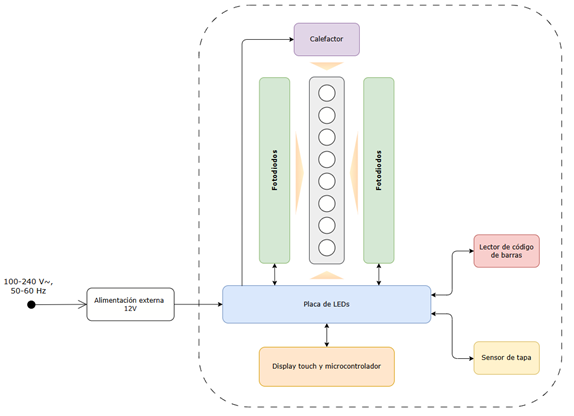
\includegraphics[width=.9\textwidth]{./Figuras/bloques.png}
\caption{Diagrama en bloques del sistema.}
\label{fig:diagBloques}
\end{figure}


\section{2. Identificación y análisis de los interesados}
\label{sec:interesados}




\begin{table}[ht]
%\caption{Identificación de los interesados}
%\label{tab:interesados}
\begin{tabularx}{\linewidth}{@{}|l|X|X|X|@{}}
\hline
\rowcolor[HTML]{C0C0C0} 
Rol           & Nombre y Apellido & Organización 	& Puesto 	\\ \hline
Cliente       & \clientename      &\empclientename	& Gerente I+D Equipos       	\\ \hline
Responsable   & \authorname       & FIUBA        	& Alumno 	\\ \hline
Orientador    & \supname	      & \pertesupname 	& Director del Trabajo Final \\ \hline
Equipo & Esteban Capuano \newline Sebastián Rodríguez dos Santos                  &  Wiener lab            	&       Diseñador mecánico \newline Jefe de Electrónica 	\\ \hline
Usuario final & Establecimientos clínicos, médicos y/o farmacéuticos                 &  -            	& -       	\\ \hline
\end{tabularx}
\end{table}

 
\begin{itemize}
	\item Cliente: Damián Lattanzi es el gerente del área de I+D Equipos en la empresa Wiener lab. Se encargará supervisar el proyecto y evaluar los resultados. También participará en la gestión de la financiación que efectúa la empresa para la realización del proyecto.  
	\item Orientador: el Esp. Ing. Gastón Vallasciani es experto en el desarrollo de firmware en sistemas embebidos y será el soporte técnico para diseñar el correspondiente al proyecto. 
	\item Equipo: el Ing. Esteban Capuano posee vasta experiencia en desarrollos mecánicos en lo que respecta equipos comerciales de laboratorio. Su conocimiento en armado de estructuras y ensambles mecánicos permitirán diseñar un esqueleto que cumpla con los requisitos del proyecto. Sebastián Rodríguez dos Santos participará en la supervisión del proyecto y brindará soporte en la definición de requerimientos y conceptos de diseño del sistema embebido.
	\item Usuario final: entidades del sector de salud o de análisis clínicos como pequeños laboratorios, farmacias, consultorios médicos, entre otros. Son aquellos que con el uso del dispositivo pueden brindar un servicio en el momento.
	
\end{itemize}



\section{3. Propósito del proyecto}
\label{sec:proposito}

El propósito del proyecto es desarrollar un equipo que permita determinar la presencia o no de un patógeno conocido en una muestra de un paciente por medio de la técnica LAMP. Además, debe otorgar el resultado en un período menor a una hora y ser fácilmente utilizable por el usuario.


\section{4. Alcance del proyecto}
\label{sec:alcance}



El proyecto incluye:
\begin{itemize}
	\item Utilización de hardware existente
	\begin{itemize}
		\item Pruebas en hardware existente para verificar su correcto funcionamiento.
	\end{itemize}
	\item Diseño y desarrollo de firmware
	\begin{itemize}
		\item Programación de microcontrolador.
		\item Programación de interfaz gráfica en pantalla táctil.
	\end{itemize}
	\item Pruebas y validación de resultados
	\item Participación en la gestión y elaboración de las partes mecánicas
		\begin{itemize}
		\item Participación en la elaboración del gabinete que unirá las partes del sistema.
	\end{itemize}
	\item Gestionar y participar en la interacción con otros sectores de la empresa
	\begin{itemize}
		\item Se pretende capacitarse y hacer seguimiento del proyecto por medio de reuniones con el departamento de Biología molecular, sector con los conocimientos necesarios para una correcta implementación de la técnica LAMP.
	\end{itemize}
	\item Documentación
	\begin{itemize}
		\item Generación de informes que exhiban resultados y validen el funcionamiento del equipo.
	\end{itemize}
	
\end{itemize}

El proyecto no incluye:

\begin{itemize}
	\item Desarrollo comercial del equipo
	\begin{itemize}
		\item No se pretende el equipo pueda ser comercializado una vez terminado el proyecto.
	\end{itemize}
	\item Producción a gran escala
	\begin{itemize}
		\item No se elabora documentación ni se desarrollan indicaciones para la producción industrial del equipo.
	\end{itemize}
		\item Capacitación o manual de usuario
	\begin{itemize}
		\item No se elabora documentación que indique como utilizar el equipo.
	\end{itemize}

	
\end{itemize}


\section{5. Supuestos del proyecto}
\label{sec:supuestos}

Para el desarrollo del presente proyecto se supone que:


\begin{itemize}
		\item La empresa proveerá de los recursos necesarios, tales como el hardware y piezas mecánicas. También brindará los reactivos químicos y las muestras biológicas necesarios para las pruebas y validación de resultados.
		\item Se asume que los integrantes del equipo, empleados de la empresa, contarán con la disponibilidad horaria necesaria para su participación en el desarrollo.
		\item Se asume que el departamento de Biología Molecular tendrá la disponibilidad para asistir a las reuniones de seguimiento y brindar capacitación.
		\item Se da por hecho que se mantiene la confidencialidad para proteger la propiedad de la empresa y que esto no será un impedimento para la evaluación, defensa y aprobación del Trabajo final de la carrera.
		\item Se da por sentado que los reactivos y la técnica LAMP a utilizar ya se encuentran estabilizados y validados por el departamento de Biología Molecular, limitando el alcance de este proyecto exclusivamente a la automatización y medición óptica.

\end{itemize}

\section{6. Requerimientos}
\label{sec:requerimientos}

En esta sección se enumeran los requerimientos del proyecto.

\begin{enumerate}
	\item Requerimientos generales:
		\begin{enumerate}
			\item El equipo debe permitir la lectura óptica simultánea e independiente de hasta 8 cubetas de reacción.
			\item El sistema óptico debe poseer 2 canales de medición (excitación/emisión) por cada cubeta.
			\item La excitación óptica debe realizarse mediante LEDs RGB con espectro de emisión específicos, seleccionando la longitud de onda según el fluoróforo utilizado.
			\item  El sistema debe contar con un módulo calefactor capaz de mantener la temperatura constante requerida por el método LAMP (típicamente entre 60 °C y 65 °C, con un error máximo a definir.
			\item El equipo debe interpretar la evolución temporal de la medición óptica para clasificar el resultado como positivo o negativo.
			\item El equipo debe contar con un puerto para comunicación y análisis de los datos.
			\item El sistema debe completar el proceso de activación, lectura y entrega de resultados en un tiempo máximo de 45 minutos.
		\end{enumerate}
	\item Requerimientos de funcionales:
		\begin{enumerate}
			\item El firmware debe sincronizar con precisión la activación de las fuentes de luz LED con la lectura del ADC de los fotodiodos. 
			\item El sistema debe implementar un lazo de control (por ejemplo, PID) para asegurar la estabilidad térmica del bloque de metal.
			\item El firmware debe mantenerse bajo control de versiones y en un repositorio privado en Gitlab o Github.		
		\end{enumerate}
	\item Requerimiento de la interfaz de usuario
	\begin{enumerate}
			\item El dispositivo debe contar con una pantalla táctil para la operación del usuario.
			\item La interfaz gráfica debe permitir configurar el modo de operación, iniciar o detener el ensayo, visualizar el estado actual y los resultados finales.
		\end{enumerate}
		\item Requerimientos de testing y validación
	\begin{enumerate}
			\item Se debe verificar el correcto funcionamiento del lazo de temperatura mediante la medición con un instrumento patrón durante un intervalo de tiempo a determinar sin variaciones fuera del rango tolerado.
			\item Se debe validar el sistema completo procesando muestras y comparando la curva de fluorescencia con la de un equipo comercial o patrón de laboratorio.
		\end{enumerate}
		\item Requerimientos de documentación
	\begin{enumerate}
			\item Se debe documentar el código fuente del firmware de manera clara.
			\item Se deben entregar los archivos de diseño de la placa de circuito impreso (PCB) y la lista de materiales (BOM).
			\item Se debe entregar la memoria técnica y el informe de avance que solicita la CESE.
		\end{enumerate}

\end{enumerate}

\section{7. Historias de usuarios (\textit{Product backlog})}
\label{sec:backlog}

A continuación se detallan las historias de usuario del proyecto, indicando el rol, la necesidad y su propósito. Se incluye también una estimación de la complejidad mediante \textit{Story Points}. Para asignar la ponderación a los \textit{Story Points}, se han establecido criterios basados en la cantidad de trabajo, la complejidad, el riesgo y la incertidumbre asociados a cada tarea.

Cantidad de trabajo a realizar:
\begin{itemize}
    \item Bajo: peso = 1
    \item Medio: peso = 5
    \item Alto: peso = 8
\end{itemize}

Complejidad del trabajo a realizar:
\begin{itemize}
    \item Bajo: peso = 1
    \item Medio: peso = 5
    \item Alto: peso = 13
\end{itemize}

Riesgo o incertidumbre del trabajo a realizar:
\begin{itemize}
    \item Bajo: peso = 5
    \item Medio: peso = 8
    \item Alto: peso = 13
\end{itemize}

Posteriormente, se realizará la sumatoria de los pesos y se tomará el valor de Fibonacci más cercano.

\begin{itemize}
    \item Como analista de laboratorio (usuario final), quiero hacer un ensayo de amplificación LAMP de forma simple y rápida, para no perder tiempo en configuraciones complejas antes de procesar la muestra.
    
    Requiere hacer pantallas, menús y botones, pero la lógica no es compleja. Sin embargo, la experiencia en ese desarrollo es muy poca.
    \begin{itemize}
    	
    	\item Cantidad: 5 
    	\item Complejidad: 1
    	\item Riesgo o incertidumbre: 5
	\end{itemize}

\begin{center}
\textit{Story point} : 13
\end{center} 
    
    \item Como analista de laboratorio, quiero visualizar el resultado final (positivo o negativo) en la pantalla de forma clara al cabo de los 45 minutos, para poder informar el diagnóstico sin necesidad de interpretar gráficos complejos.
    
     Requiere procesar datos y generar curvas para su interpretación. Cualquier ruido óptico o error en la lectura afecta directamente.
	\begin{itemize}
    	\item Cantidad: 1 
    	\item Complejidad: 13
    	\item Riesgo o incertidumbre: 5
	\end{itemize}

\begin{center}
\textit{Story point} : 21
\end{center}
    
    \item Como investigador del departamento de Biología Molecular (Wiener lab), quiero que el equipo guarde un registro temporal con las curvas de fluorescencia en la memoria, para poder exportar los datos a una PC y analizar la cinética de la reacción.
    
    Guardar datos integrando un sistema de archivos (SD) es complejo y lleva tiempo. Esta escritura o lectura no debe bloquear el proceso principal del equipo.
    \begin{itemize}
    	\item Cantidad: 8
    	\item Complejidad: 13
    	\item Riesgo o incertidumbre: 13
	\end{itemize}

\begin{center}
\textit{Story point} : 34
\end{center} 
    
    \item Como ingeniero de desarrollo, quiero disponer de un puerto USB y comandos de depuración (\textit{debug}), para poder monitorear en tiempo real las lecturas de los fotodiodos y el estado del lazo PID de temperatura durante la etapa de desarrollo. 
    
    Implementar un puerto serie para comandos es algo ya desarrollado y muy directo en microcontroladores. 
    \begin{itemize}
    	\item Cantidad: 5
    	\item Complejidad: 5
    	\item Riesgo o incertidumbre: 5
	\end{itemize}

\begin{center}
\textit{Story point} : 13
\end{center}

\end{itemize}


\section{8. Entregables principales del proyecto}
\label{sec:entregables}

Los entregables del proyecto son:

\begin{itemize}
	\item Prototipo funcional: hardware electrónico (placas de detección y control) ensamblado y operativo junto con el gabinete mecánico preliminar.
	\item Archivos de diseño de hardware: diagramas esquemáticos, diseño de circuito impreso (archivos Gerber) y lista de materiales (BOM).
	\item Código fuente del firmware: repositorios con el código implementado para el microcontrolador y para la interfaz gráfica de la pantalla táctil.
	\item Informes de validación: documentos que detallen los resultados de las pruebas de estabilidad térmica y las mediciones ópticas de fluorescencia realizadas.
	\item Memoria del Trabajo Final: documento académico final requerido para la aprobación de la Carrera de Especialización en Sistemas Embebidos.
\end{itemize}

\section{9. Desglose del trabajo en tareas}
\label{sec:wbs}

\begin{enumerate}


\item Investigación y análisis preliminar (50 h)
	\begin{enumerate}
	\item Estudio detallado de la técnica LAMP, requerimientos térmicos y ópticos. (40 h)
	\item Análisis de normativas de seguridad eléctrica aplicables en laboratorio. (10 h)
	\end{enumerate}
	
\item Planificación y gestión del proyecto (55 h)
	\begin{enumerate}
	\item Elaboración y corrección del plan de proyecto. (20 h)
	\item Reuniones periódicas de seguimiento y revisión con el director y el equipo. (25 h)
	\item Revisión y ajustes de planificación. (10 h)
	\end{enumerate}


\item Desarrollo e integración (325 h)
	\begin{enumerate}
	\item Configuración de entorno de desarrollo. (20 h)
	\item Configuración inicial de periféricos y \textit{drivers} de bajo nivel. (45 h)
	\item Aplicación de almacenamiento temporal en memoria MicroSD. (30 h)
	\item Desarrollo de comunicación serie y exportación de datos (USB). (30 h)
	\item Implementación del lazo de control PID para la estabilización de temperatura. (30 h)
	\item Programación de la interfaz gráfica de usuario en la pantalla táctil. (30 h)
	\item Integración del hardware con las partes mecánicas y el gabinete preliminar. (10 h)
	\item Integración de control térmico con excitación óptica y lectura. (40 h)
	\item Integración de almacenamiento de datos de lecturas en SD. (30 h)
	\item Integración de exportación de datos almacenados en SD. (30 h)
	\item Desarrollo del algoritmo de análisis de la curva para el diagnóstico. (30 h)
	\end{enumerate}

\item Pruebas y validación (90 h)
	\begin{enumerate}
	\item Pruebas del dispositivo con ensayos biológicos funcionales reales aplicando la técnica LAMP. (50 h)
	\item Ajustes de firmware y/o hardware. (40 h)
	\end{enumerate}

\item Documentación final (80 h)
	\begin{enumerate}
	\item Redacción de los informes de validación. (15 h)
	\item Redacción de la Memoria del Trabajo Final e informe de avance. (45 h)
	\item Preparación de diapositivas y ensayo para la defensa pública. (20 h)
	\end{enumerate}
\end{enumerate}

Cantidad total de horas: 600 h.

\begin{landscape}

\section{10. Diagrama de Activity On Node}
\label{sec:AoN}

\vspace*{4cm}

\begin{figure}[h]
\centering 
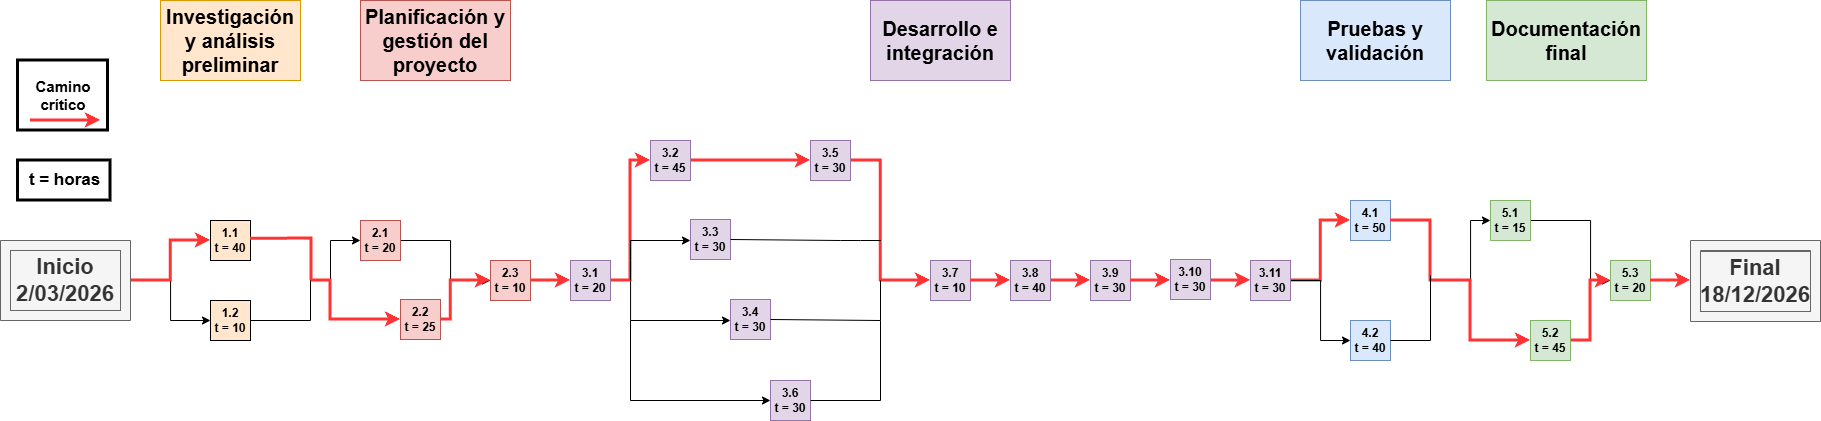
\includegraphics[width=1.55\textwidth]{./Figuras/AoN_GdP_Gianchino.png}
\caption{Diagrama de \textit{Activity on Node}.}
\label{fig:AoN}
\end{figure}

\end{landscape}

\begin{landscape}
\section{11. Diagrama de Gantt}
\label{sec:gantt}

\begin{figure}[h]
\centering 
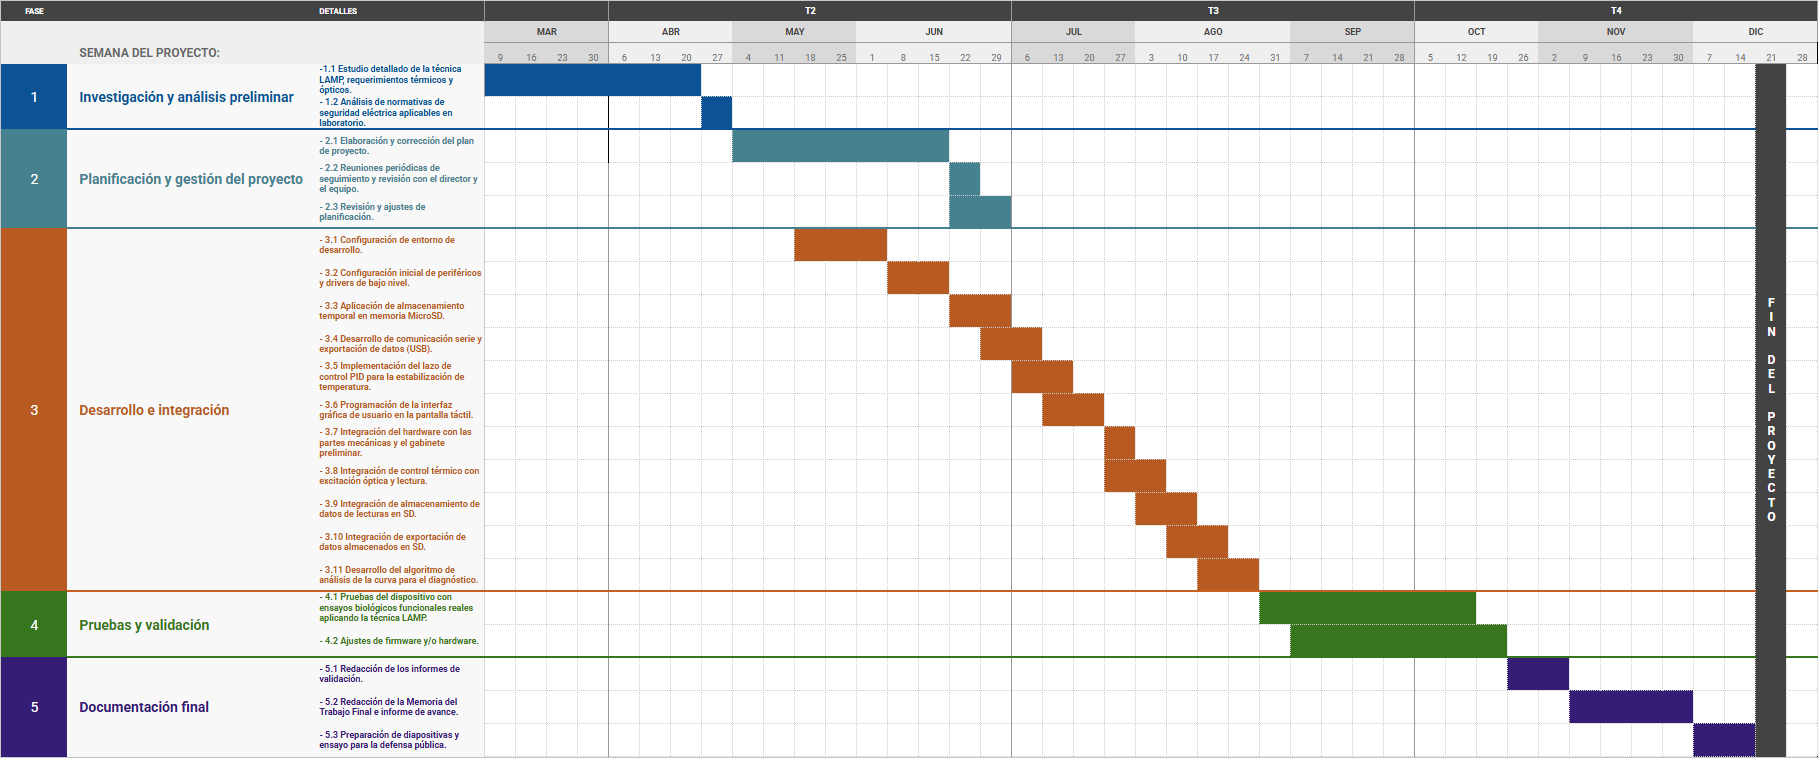
\includegraphics[width=1.57\textwidth]{./Figuras/gantt.png}
\caption{Diagrama de \textit{Gantt}.}
\label{fig:AoN}
\end{figure}

\end{landscape}
\section{12. Presupuesto detallado del proyecto}
\label{sec:presupuesto}

\begin{consigna}{red}
Si el proyecto es complejo entonces separarlo en partes:
\begin{itemize}
	\item Un total global, indicando el subtotal acumulado por cada una de las áreas.
	\item El desglose detallado del subtotal de cada una de las áreas.
\end{itemize}

IMPORTANTE: No olvidarse de considerar los COSTOS INDIRECTOS.

Incluir la aclaración de si se emplea como moneda el peso argentino (ARS) o si se usa moneda extranjera (USD, EUR, etc). Si es en moneda extranjera se debe indicar la tasa de conversión respecto a la moneda local en una fecha dada.

\end{consigna}

\begin{table}[htpb]
\centering
\begin{tabularx}{\linewidth}{@{}|X|c|r|r|@{}}
\hline
\rowcolor[HTML]{C0C0C0} 
\multicolumn{4}{|c|}{\cellcolor[HTML]{C0C0C0}COSTOS DIRECTOS} \\ \hline
\rowcolor[HTML]{C0C0C0} 
Descripción &
  \multicolumn{1}{c|}{\cellcolor[HTML]{C0C0C0}Cantidad} &
  \multicolumn{1}{c|}{\cellcolor[HTML]{C0C0C0}Valor unitario} &
  \multicolumn{1}{c|}{\cellcolor[HTML]{C0C0C0}Valor total} \\ \hline
 &
  \multicolumn{1}{c|}{} &
  \multicolumn{1}{c|}{} &
  \multicolumn{1}{c|}{} \\ \hline
 &
  \multicolumn{1}{c|}{} &
  \multicolumn{1}{c|}{} &
  \multicolumn{1}{c|}{} \\ \hline
\multicolumn{1}{|l|}{} &
   &
   &
   \\ \hline
\multicolumn{1}{|l|}{} &
   &
   &
   \\ \hline
\multicolumn{3}{|c|}{SUBTOTAL} &
  \multicolumn{1}{c|}{} \\ \hline
\rowcolor[HTML]{C0C0C0} 
\multicolumn{4}{|c|}{\cellcolor[HTML]{C0C0C0}COSTOS INDIRECTOS} \\ \hline
\rowcolor[HTML]{C0C0C0} 
Descripción &
  \multicolumn{1}{c|}{\cellcolor[HTML]{C0C0C0}Cantidad} &
  \multicolumn{1}{c|}{\cellcolor[HTML]{C0C0C0}Valor unitario} &
  \multicolumn{1}{c|}{\cellcolor[HTML]{C0C0C0}Valor total} \\ \hline
\multicolumn{1}{|l|}{} &
   &
   &
   \\ \hline
\multicolumn{1}{|l|}{} &
   &
   &
   \\ \hline
\multicolumn{1}{|l|}{} &
   &
   &
   \\ \hline
\multicolumn{3}{|c|}{SUBTOTAL} &
  \multicolumn{1}{c|}{} \\ \hline
\rowcolor[HTML]{C0C0C0}
\multicolumn{3}{|c|}{TOTAL} &
   \\ \hline
\end{tabularx}%
\end{table}


\section{13. Gestión de riesgos}
\label{sec:riesgos}

\begin{consigna}{red}
a) Identificación de los riesgos (al menos cinco) y estimación de sus consecuencias:
 
Riesgo 1: detallar el riesgo (riesgo es algo que si ocurre altera los planes previstos de forma negativa)
\begin{itemize}
	\item Severidad (S): mientras más severo, más alto es el número (usar números del 1 al 10).\\
	Justificar el motivo por el cual se asigna determinado número de severidad (S).
	\item Probabilidad de ocurrencia (O): mientras más probable, más alto es el número (usar del 1 al 10).\\
	Justificar el motivo por el cual se asigna determinado número de (O). 
\end{itemize}   

Riesgo 2:
\begin{itemize}
	\item Severidad (S): X.\\
	Justificación...
	\item Ocurrencia (O): Y.\\
	Justificación...
\end{itemize}

Riesgo 3:
\begin{itemize}
	\item Severidad (S):  X.\\
	Justificación...
	\item Ocurrencia (O): Y.\\
	Justificación...
\end{itemize}


b) Tabla de gestión de riesgos:      (El RPN se calcula como RPN=SxO)

\begin{table}[htpb]
\centering
\begin{tabularx}{\linewidth}{@{}|X|c|c|c|c|c|c|@{}}
\hline
\rowcolor[HTML]{C0C0C0} 
Riesgo & S & O & RPN & S* & O* & RPN* \\ \hline
       &   &   &     &    &    &      \\ \hline
       &   &   &     &    &    &      \\ \hline
       &   &   &     &    &    &      \\ \hline
       &   &   &     &    &    &      \\ \hline
       &   &   &     &    &    &      \\ \hline
\end{tabularx}%
\end{table}

Criterio adoptado: 

Se tomarán medidas de mitigación en los riesgos cuyos números de RPN sean mayores a...

Nota: los valores marcados con (*) en la tabla corresponden luego de haber aplicado la mitigación.

c) Plan de mitigación de los riesgos que originalmente excedían el RPN máximo establecido:
 
Riesgo 1: plan de mitigación (si por el RPN fuera necesario elaborar un plan de mitigación).
  Nueva asignación de S y O, con su respectiva justificación:
  \begin{itemize}
	\item Severidad (S*): mientras más severo, más alto es el número (usar números del 1 al 10).
          Justificar el motivo por el cual se asigna determinado número de severidad (S).
	\item Probabilidad de ocurrencia (O*): mientras más probable, más alto es el número (usar del 1 al 10).
          Justificar el motivo por el cual se asigna determinado número de (O).
	\end{itemize}

Riesgo 2: plan de mitigación (si por el RPN fuera necesario elaborar un plan de mitigación).
 
Riesgo 3: plan de mitigación (si por el RPN fuera necesario elaborar un plan de mitigación).

\end{consigna}


\section{14. Gestión de la calidad}
\label{sec:calidad}

\begin{consigna}{red}
Elija al menos diez requerimientos que a su criterio sean los más importantes/críticos/que aportan más valor y para cada uno de ellos indique las acciones de verificación y validación que permitan asegurar su cumplimiento.

\begin{itemize} 
\item Req \#1: copiar acá el requerimiento con su correspondiente número.

\begin{itemize}
	\item Verificación para confirmar si se cumplió con lo requerido antes de mostrar el sistema al cliente. Detallar.
	\item Validación con el cliente para confirmar que está de acuerdo en que se cumplió con lo requerido. Detallar. 
\end{itemize}

\end{itemize}

Tener en cuenta que en este contexto se pueden mencionar simulaciones, cálculos, revisión de hojas de datos, consulta con expertos, mediciones, etc.  

Las acciones de verificación suelen considerar al entregable como ``caja blanca'', es decir se conoce en profundidad su funcionamiento interno.  

En cambio, las acciones de validación suelen considerar al entregable como ``caja negra'', es decir, que no se conocen los detalles de su funcionamiento interno.

\end{consigna}

\section{15. Procesos de cierre}    
\label{sec:cierre}

\begin{consigna}{red}
Establecer las pautas de trabajo para realizar una reunión final de evaluación del proyecto, tal que contemple las siguientes actividades:

\begin{itemize}
	\item Pautas de trabajo que se seguirán para analizar si se respetó el Plan de Proyecto original:\\
	 - Indicar quién se ocupará de hacer esto y cuál será el procedimiento a aplicar. 
	\item Identificación de las técnicas y procedimientos útiles e inútiles que se emplearon, los problemas que surgieron y cómo se solucionaron:\\
	 - Indicar quién se ocupará de hacer esto y cuál será el procedimiento para dejar registro.
	\item Indicar quién organizará el acto de agradecimiento a todos los interesados, y en especial al equipo de trabajo y colaboradores:\\
	  - Indicar esto y quién financiará los gastos correspondientes.
\end{itemize}

\end{consigna}

\end{document}
